%!TEX root = ../Main.tex

\chapter{PolyMarker: A fast polyploid primer design pipeline}
\chaptermark{PolyMarker}
\label{cha:polymarker}
%\section{Introduction} 
%Explain how the SNP markers are designed without the tool and an overview. 

In modern breeding programs SNP markers are a prevalent technology to select seeds containing a particular locus linked to a trait (ie. a marker linked to a resistance gene, see Chapter \ref{yr15}). 
SNP marker are an specific case of \gls{pcr} amplification with two competing sequences from different alleles are amplified. 


In general, \acrshort{pcr} amplification is a technique that can be used to copy several times a fragment of DNA. 
To start the amplification a pair of sequences (left and right primers) on each side of the target sequence is required. 
The sequence between primers is copied thanks to the DNA polymerase, an enzyme that moves along the DNA strand making a copy (product). 
The process starts when the DNA molecule is melted in individual strands with an increase of temperature. 
Then, the temperature is dropped so the primers anneal to the DNA strands. 
At this point, the polymerase starts extending the strand from the 3'-end of the primer. 
The temperature is raised again to separate the new strand from the original DNA and lowered again to get the right primer to anneal to the new product.
Then, in the extension step, the amplification occurs until the end of template sequence, were the 5'-end of the left primer was originally located. 
This process is repeated several times to increase the representation of the target DNA (Figure \ref{fig:poly:amplificationProduct}).  

\begin{figure}

\includegraphics[width=1\textwidth]{PolyMarker/Figures/intro/amplificationProduct.pdf}
\caption{PCR is used to amplify a region of the DNA (green bar). To target to amplify (product; red line) is found by a pair of primers (blue lines). The 3' and 5' represent the orientation of the primers.}
\label{fig:poly:amplificationProduct}
\end{figure}

A technology used for SNP markers is KASP. 
The assays consists on triplets of primers, having a primer for each allele and a common primer that will amplify regardless of the allele. 

The allelic primers have at the 5'-end a tail, HEX (5' GAAGGTCGGAGTCAACGGATT 3') or FAM (5' GAAGGTGACCAAGTTCATGCT 3'), which is used to distinguish between them (Figure \ref{fig:poly:kaspTriplet}). 
The KASP mix contains complementing oligos to the HEX and FAM tail, which contain a dye that is only visible when the corresponding allele has amplified. 
The intensity of each dye is used to measure relative amplification of each allele. 
On KASP assays, the distance between the left and right primers is as short as possible, to avoid having an extension step. 
As the primers are around 21-25bp, the minimum product size is between 42-50bp, with products rarely going over 75bp.  
Samples with the same genotype cluster: Samples on each axis correspond to homozygous individuals and samples clustered between the homozygous clusters are heterozygous (Figure \ref{fig:poly:kaspHet}). 
If the experiment failed, because poor amplification or because all the samples have the same genotype, there are no distinguishable clusters (Figure \ref{fig:poly:kaspFail}; \citealt{LGC}).


\begin{figure}
\centering
    \begin{subfigure}{0.85\textwidth}
    \caption{}
    \label{fig:poly:kaspTriplet}
    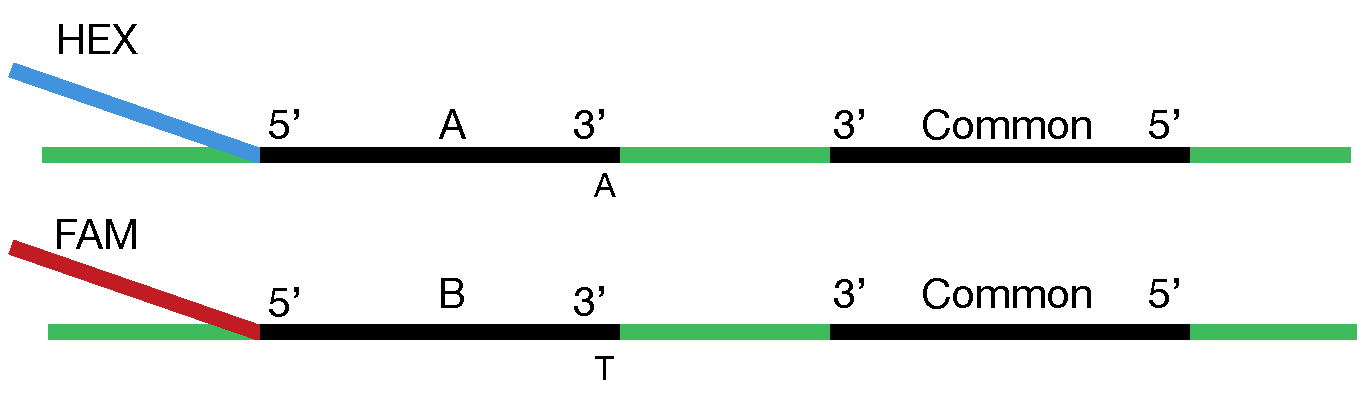
\includegraphics[width=1\textwidth]{PolyMarker/Figures/intro/kaspTriplet.pdf}
    \end{subfigure}

    \begin{subfigure}{0.45\textwidth}
    \caption{}
    \label{fig:poly:kaspHet}
    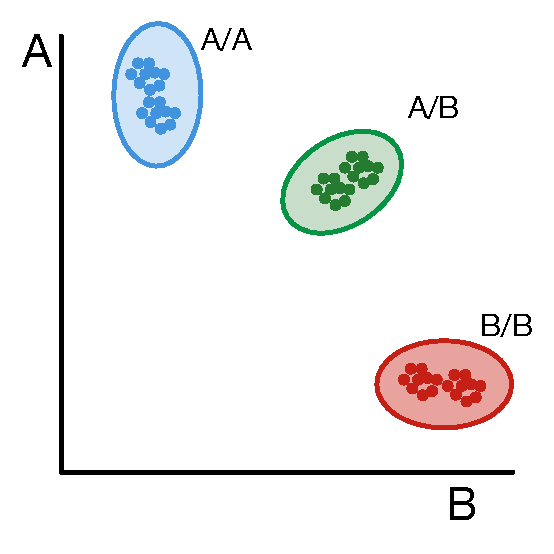
\includegraphics[width=1\textwidth]{PolyMarker/Figures/intro/kaspHet.pdf}
    \end{subfigure}
    ~
    \begin{subfigure}{0.45\textwidth}
    \caption{}
    \label{fig:poly:kaspFail}
    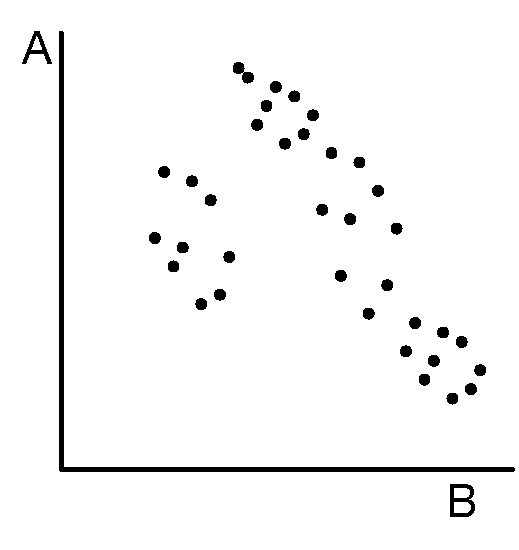
\includegraphics[width=1\textwidth]{PolyMarker/Figures/intro/kaspFail.pdf}
    \end{subfigure}

\caption{Kasp Assays (\subref{fig:poly:kaspTriplet}) A KASP assay consists on three primers. Primers A and B are specific for certain allele and the HEX and FAM tails are added at the 5'-end on each primer. The common primer amplifies both possible products. The SNP is an A/T, the only difference between alleles. (\subref{fig:poly:kaspHet}) Ideal KASP results of samples containing only homozaygous samples. The samples containing  A allele clusters on the top-left (blue), the B allele cluster on the bottom-right (red) and the heterozygous cluster between the homozygous clusters (green). Each dot represent a sample and the axes are the relative intensity of amplification of each allele. (\subref{fig:poly:kaspFail}) KASP results of a failed experiment were clear clusters between samples are missing. }
\end{figure}


One of the main challenges of working with polyploid species is the design of genome specific molecular markers. 
On hexaploid wheat, most of the genes have at three homoeologues copies, one for each genome (See section \ref{lit:polyploidy}). 
The similarity between homoeologues is around 98\%, which represent around 1 mismatch for every 50 bp. 
This means that a primer in a conserved region of 21 bases target any of the homoeologues if it doesn't have variations on it.
In Figure \ref{fig:poly:pimerChrSpecificDiagram}, variations between genomes are represented with red lines, which are randomly distributed across homoeologues. 
The $\alpha$ is randomly generated using the sequence of chromosome 1D, however, because it doesn't have any variation specific to the D genome, products from it can amplify any of the genome. 
On the contrary, the $\beta$ starts with a base that has a base that is unique to the D genome, hence the product is genome specific. 

\begin{figure}
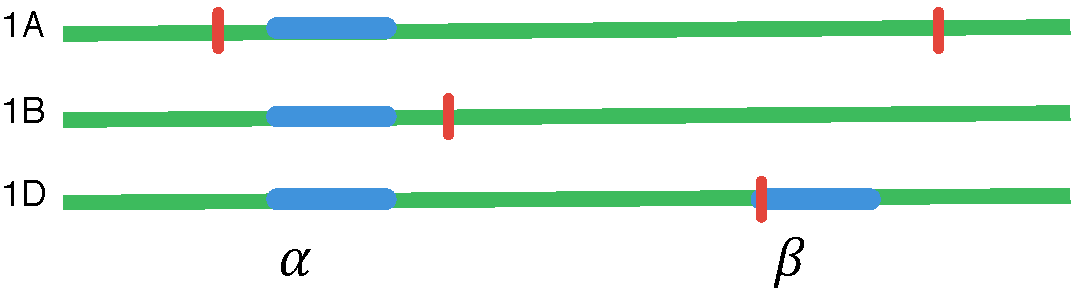
\includegraphics[width=1\textwidth]{PolyMarker/Figures/intro/primerChrSpecificDiagram.pdf}
\caption{Primers selected randomly (blue lines) can bind to any of the three homoeologous regions if they fall on regions without variations between them (red vertical lines). The $\alpha$ primer doesn't contain any variation between chromosomes, hence it will bind to the chromosomes 1A, 1B and 1D. The $\beta$ primer has a variation specific to the D genome, hence it will only amplify the 1D chromosome.}
\label{fig:poly:pimerChrSpecificDiagram}
\end{figure}

A variation between homoeologues in the primers is not enough to guarantee that the amplification is going to be genome specific. 
The polymerase is more sensible to variations were the amplification starts, so variations in the 3'-end improve the specificity of primers \citep{Huang2010}. 
Hence, when designing genome-specific assays the specificitt of the primers is scored according to the position of the variation as:  strong, when the variation is on the 3'-end; OK, when the variation is on the 2nd positionl no too strong when the variation is on the 3rd position and; not specific when the variation occurs after the 3rd position (Figure \ref{fig:poly:3PrimeRules}).  

\begin{figure}
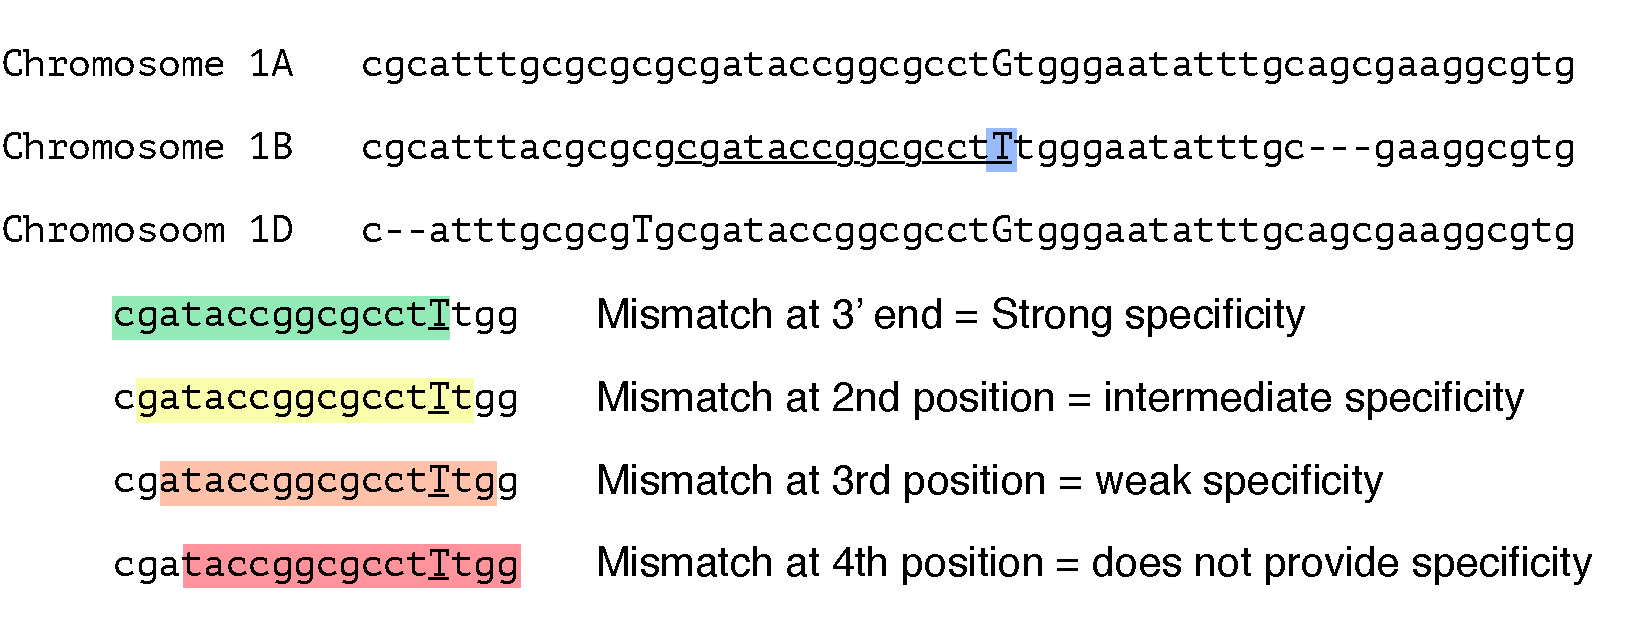
\includegraphics[width=1\textwidth]{PolyMarker/Figures/intro/specificPosition.pdf}
\caption{Several candidates to design a genome specific primer for chromosome 1B. The T highlighted in blue is a variation unique to the target chromosome. The closer the T providing specificity is to the 3' of the primer, the more specific it is. }
\label{fig:poly:3PrimeRules}
\end{figure}


To ensure that all the constrains needed to produce pairs, the following steps need to be done: 

\begin{enumerate}
\item First, a global alignment of the target sequence is used to find all the homoeologues and paralogues in the reference genome.
This is done with tools like \verb|blast| \citep{Altschul1990}, \verb|blat| \citep{Kent2002} or \verb|exonerate| \citep{Slater2005}.
All this tools take a reference sequence and make some sort of index to speed up the search of the queried sequence  \ref{fig:poly:globalSearch}. 
The results are aligned to the target, but not between them. 
\item To put all the sequences in the appropriate context, a local alignment is done (Figure \ref{fig:poly:globalAround}). 
This is done by extracting all the hits to the target reference and using a program like \verb|mafft| \citep{Katoh2013} or \verb|clustal| \citep{Higgins1988}. 
This tools are based on aligning all the possible sequences in pairs all the possible pairs.
The distance between pairs is calculated to find which sequences are closer to each other, and then the process is repeated to refine the alignments until a consensus alignment is reached. 
This is useful on the context of genome-specific primer design because to correct the alignment on the presence of small \gls{indels}.  
\item Finally, the primers are validated to conform physiochemical properties that ensure the amplification. 
The melting temperature needs to be in the range were the DNA will separate, but not too high that reaching the temperature will damage other elements in the reaction, such as the polymerase. 
Also, the primers must avoid sequences that self-bind, hairpins, or binding to the complementary primer. 
The validation primers based on their intrinsic properties can be done with tools like \verb|Primer3| \citep{Rozen}. 
\unsure{If possible, expand and add diagram}
\end{enumerate}

\begin{figure}
\begin{subfigure}[b]{0.6\textwidth}
\caption{}
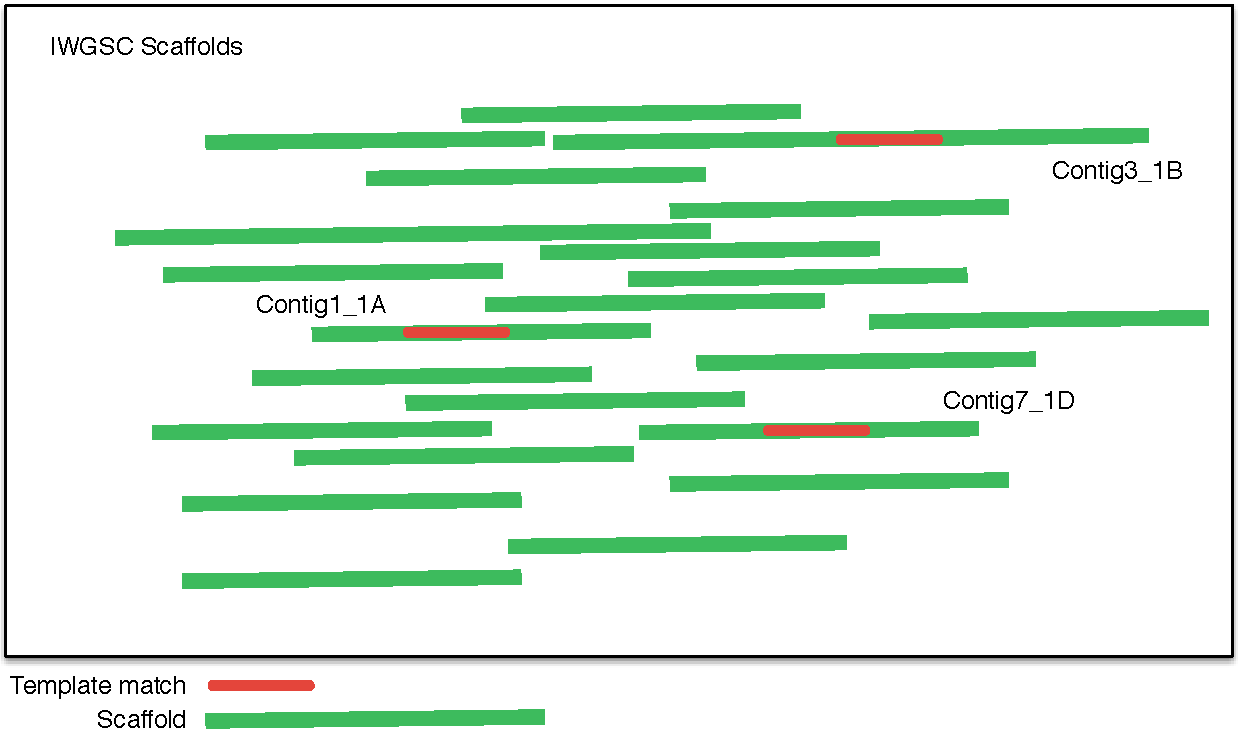
\includegraphics[width=1\textwidth]{PolyMarker/Figures/aln/scaffoldsSearch.pdf}
\label{fig:poly:globalSearch}
\end{subfigure}
~
\begin{subfigure}[b]{0.35\textwidth}
\caption{}
\raisebox{12ex}{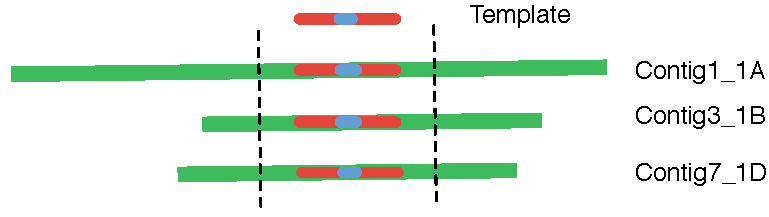
\includegraphics[width=1\textwidth]{PolyMarker/Figures/aln/scaffoldsFoundAround.pdf}}
\label{fig:poly:globalAround} 
\end{subfigure}
\caption{(\subref{fig:poly:globalSearch}) Global search of templates in the reference contigs. (\subref{fig:poly:globalAround}) Selected regions around the SNP on every chromosome. The blue line represents the position of the SNP.}
\end{figure}

Since most of the steps required to design genome-specific primers require different bioinformatic tools and the rules to improve the efficiency of the primers are established, I hypothesize that it is possible to automate the process. 
On that premise, I developed PolyMarker, a pipeline that takes the reference genome and a list of \acrshortpl{snp} and produces genome-specific primers \citep{Ramirez-Gonzalez2015a}. 

\section{Pipeline}
PolyMarker is an automated pipeline that takes as input a list of SNPs and a reference file and produces a list of primer triplets for SNP genotyping. 
The list of SNPs is first converted to a \verb|FASTA| file with ambiguity codes \citep{Cornish-Bowden1985} 
The template sequences are aligned with \verb|exonerate| \citep{Slater2005}  to find the homoeologous regions to the target sequence. 
Then, the alignment between homoeologues is refined using \verb|MAFFT| \citep{Katoh2013}. 
A list of candidate variations is produced and used as input for \verb|Primer3| \citep{Rozen}. 
Finally, the output of \verb|Primer3| is parsed to find the best primer pair that contains a the targeted SNP and a base that is specific to the target genome (Figure \ref{fig:poly:pipeline}).  
The pipeline is written as a Ruby script, using parsers and wrappers from BioRuby \citep{Goto2010} and bio-samtools \citep{Etherington2015,Ramirez-Gonzalez2012}. 
The software is open source and released as a biogem \citep{Bonnal2012}, \verb|bio-polyploid-tools|, the source code is available in github: \verb|https://github.com/TGAC/bioruby-polyploid-tools|.

\begin{figure}
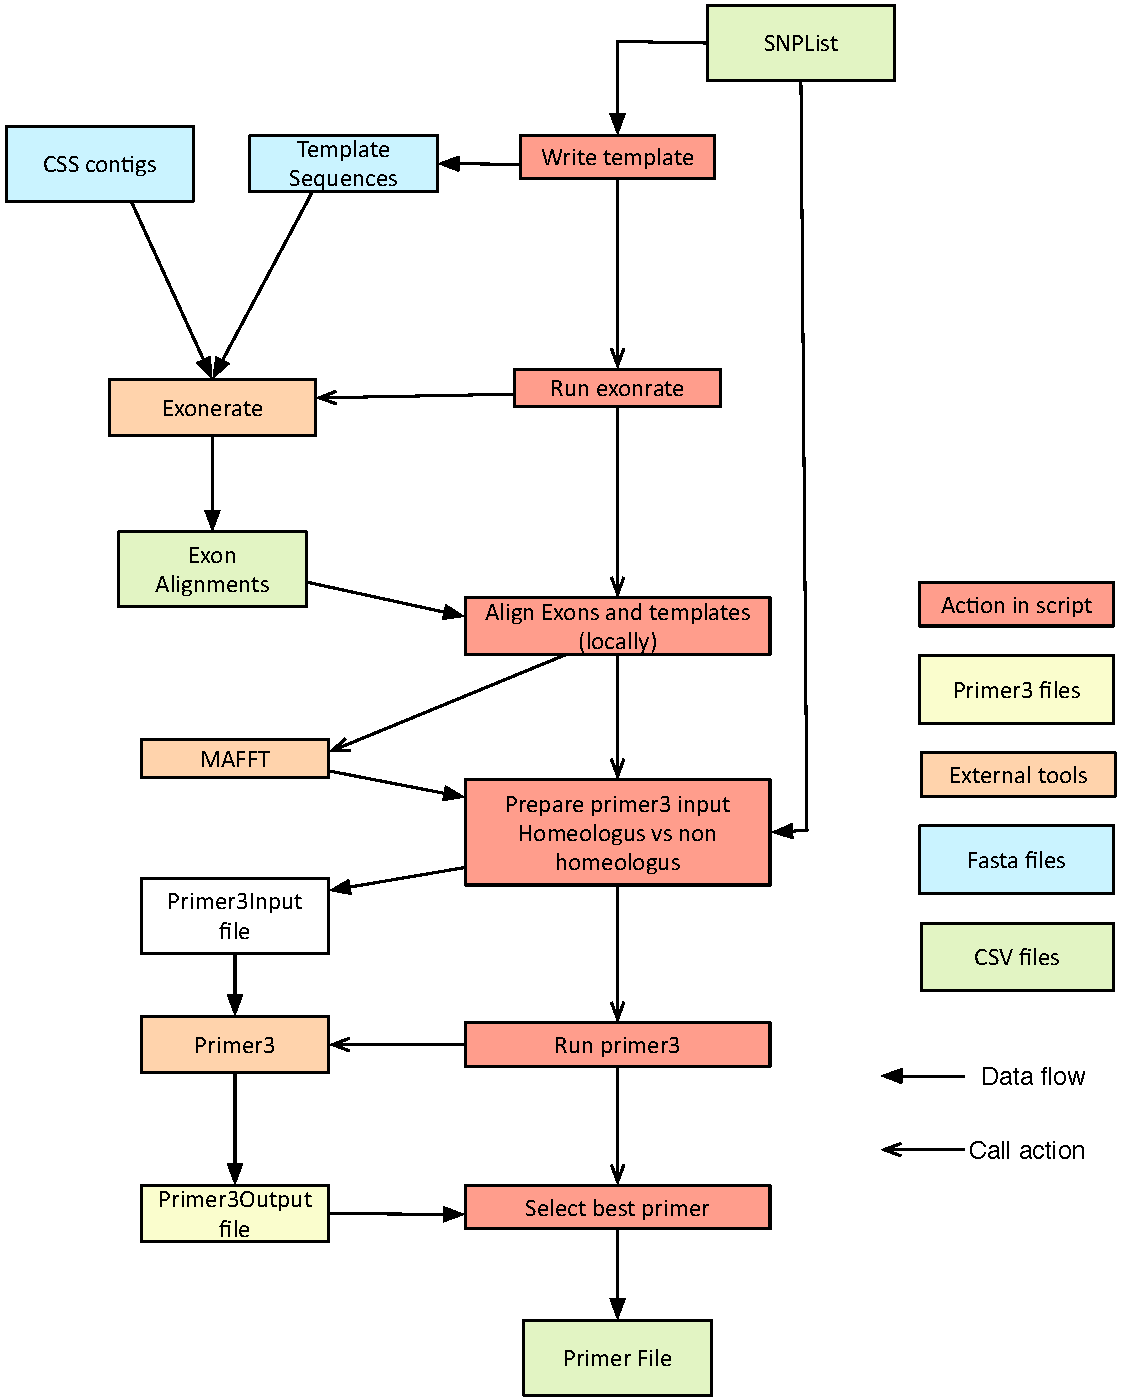
\includegraphics[width=1\textwidth]{PolyMarker/Figures/pipeline.pdf}
        \caption{Steps and tools called by PolyMarker. The colour of the boxes represent: the step is an action inside the script(red); actions of the script(light red); temporary files(yellow); inputs(blue) and; outpus(green)}
        \label{fig:poly:pipeline}
\end{figure}

The PolyMarker input consists on SNP list with: unique name for the marker, the target chromosome and the sequence for the marker. 
The alternative alleles are surrounded by square brackets within the sequence. PolyMarker can take a list of several markers and design them in batch (Figure \ref{fig:poly:input}). 
A \verb|FASTA| file is produced with all the template sequences, with the alternative alleles substituted by the IUAPC ambiguity codes \citep{Cornish-Bowden1985}. 
The flanking sequence surrounding the SNP is limited by default to 100bp to reduce the search time and avoid missing regions that diverge near the SNP, as when the variation is near an intron-exon junction. 
%%TODO: Should we elaborate more here? 

\begin{figure}
    \centering
    \begin{subfigure}[b]{0.8\textwidth}
        \caption{}
        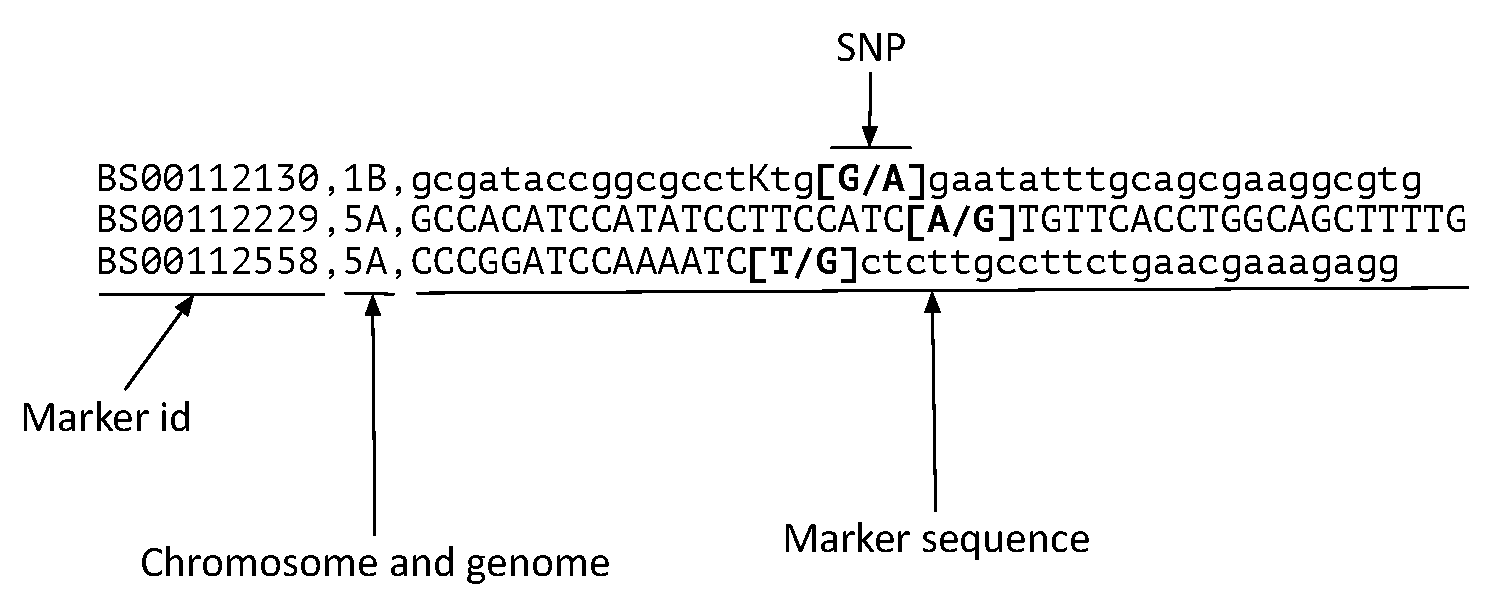
\includegraphics[width=1\textwidth]{PolyMarker/Figures/aln/input.pdf} 
        \label{fig:poly:input}
    \end{subfigure}

    
    \begin{subfigure}[b]{0.4\textwidth}
        \caption{}
        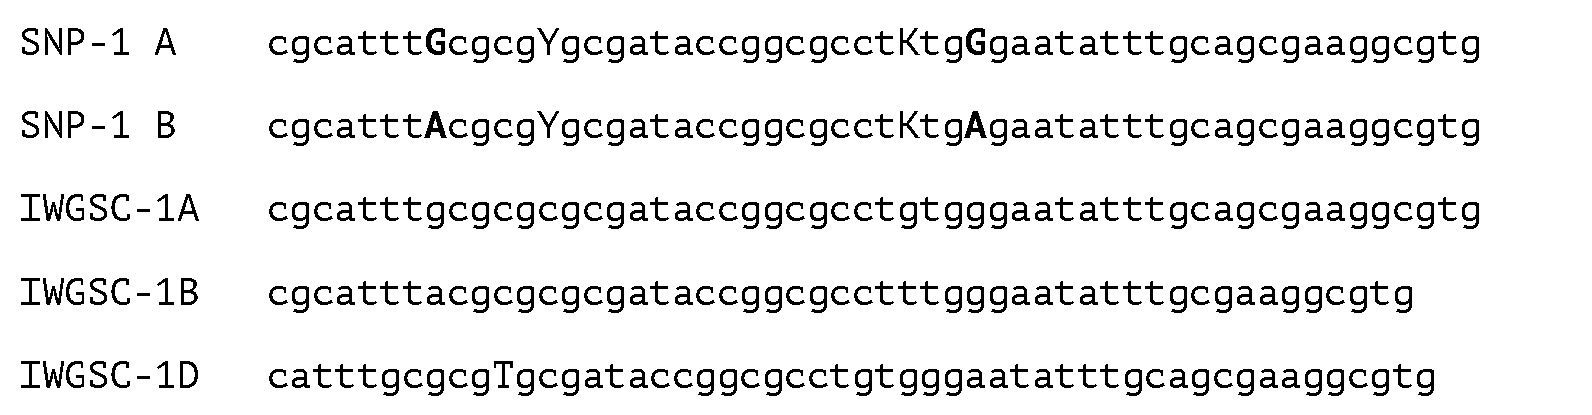
\includegraphics[width=1\textwidth]{PolyMarker/Figures/aln/scaffoldsFound.pdf}
        \label{fig:poly:globalSequence}
    \end{subfigure}
    ~ %add desired spacing between images, e. g. ~, \quad, \qquad, \hfill etc. 
      %(or a blank line to force the subfigure onto a new line)
    \begin{subfigure}[b]{0.4\textwidth}
        \caption{}
        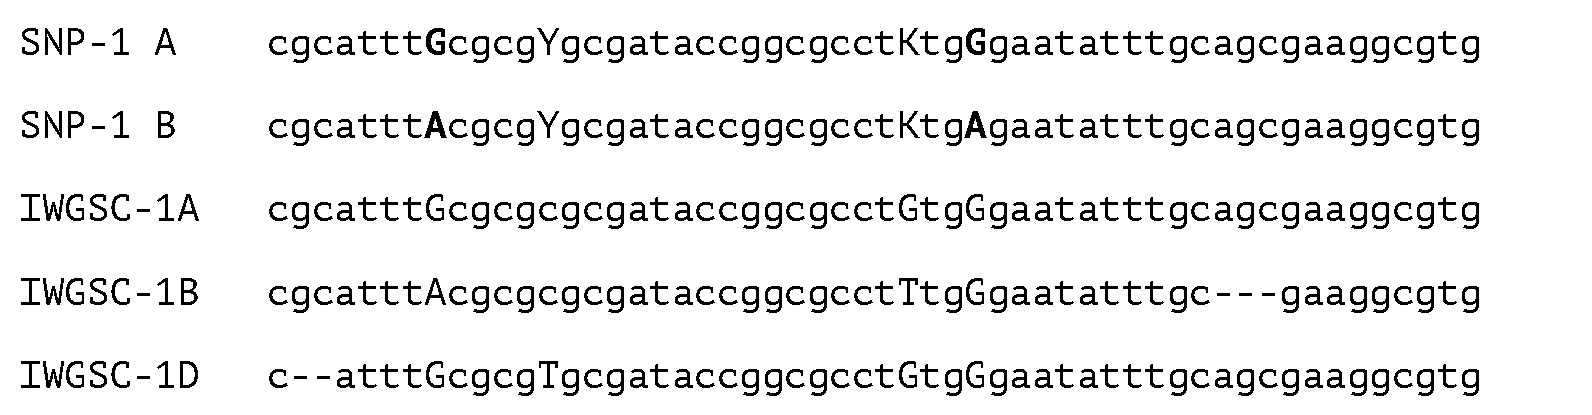
\includegraphics[width=1\textwidth]{PolyMarker/Figures/aln/localAlignment.pdf}
        \label{fig:poly:localSequence}
    \end{subfigure}

    \begin{subfigure}[b]{0.8\textwidth}
        \caption{}
        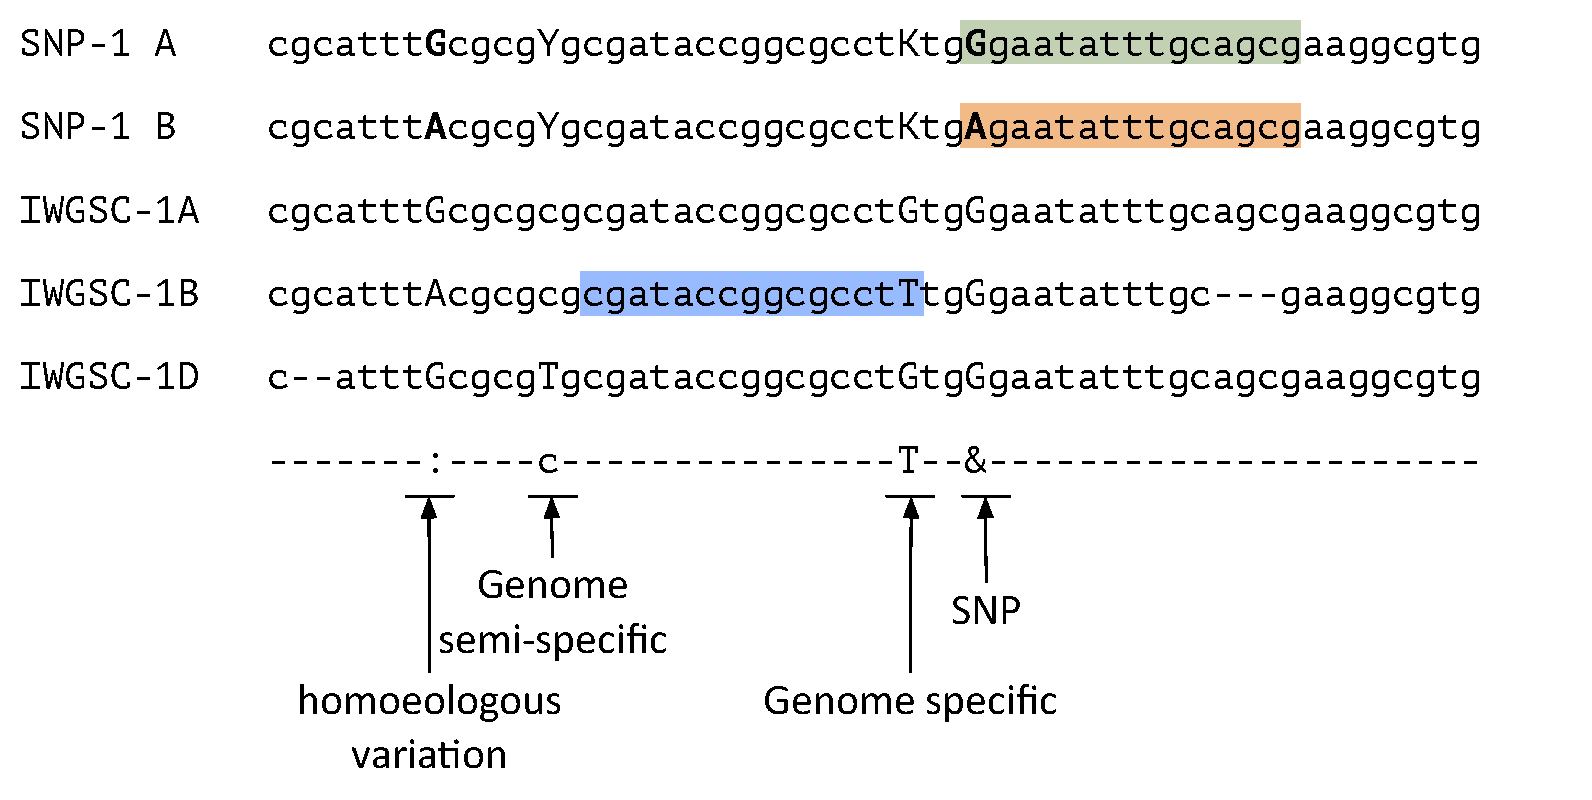
\includegraphics[width=1\textwidth]{PolyMarker/Figures/aln/mask.pdf} 
        \label{fig:poly:mask}
    \end{subfigure}
    \caption{Alignments done by PolyMarker.(\subref{fig:poly:input}) input. The alternative alleles are sorrounded by brackets.(\subref{fig:poly:globalSequence}) Sequence of found regions around the SNP. (\subref{fig:poly:localSequence}) Local alignment on regions around the SNP detects indels. (\subref{fig:poly:mask}) Alignment with mask and primer candidates.}
    \label{fig:global}
\end{figure}

The template sequences are aligned to the reference using \verb|exonerate| (\citealt{Slater2005}; Figure \ref{fig:poly:globalSearch}). 
The alignment is refined with the \verb|--model est2genome| option, to allow the search of sequences coming from transcripts, a common source of SNPs \citep{Allen2011}. 
The exonerate output is formatted with the \verb|--ryo| (roll your own format) to get an output easy to parse. 
All the hits that contain the SNP are extracted from the reference with a flanking sequence that extend out of the hit, by defualt, to 100bp on each side of the SNP, Figure \ref{fig:poly:globalAround}.
The size of the flanking sequence can be set to different sizes to allow the design of different types of primers. 
Different homoeologues may contain small indels, Figure \ref{fig:poly:globalSequence}. 
To enable a comparasion base-per-base, a local alignment with \verb|MAFFT| \citep{Katoh2013} is produced, Figure \ref{fig:poly:localSequence}. 

PolyMarker searches across each base in the local alignment to identify the variations across homoeologues and the target marker.
A mask is produced to highlight the bases with a variations, Figure \ref{fig:poly:mask}, on the following categories:
\begin{labeling}{Non-homoeologous}
%\begin{description}[align=right,labelwidth=4cm]
\item [Specific] Homoeologous polymorphism which is only present in the target genome (upper case).
\item [Semi-specific] Homoeologous polymorphism which is found in 2 of the 3 genomes, hence it discriminates against one of the off-target genomes or when not all the homoeologous sequences were found (lower case).
\item [Non-specific] No variation is found across homoeologues (\texttt{-}).
\item [Homoeologous] The target SNP is present across different chromosomes, so candidate SNP markers on this category are not expected to be reliably identify the allele (\texttt{:}).
\item [Non-homoeologous] The target SNP is not present across chromosomes, so it can be used to identify an allele (\texttt{\&}).
%\end{description} 
\end{labeling} 

PolyMarker was designed to produce SNP assays for KASP genotyping \citep{LGC}, which requires a common primer and two allele-specific primers. 
The common primer is selected to start on a position from a: Specific; Semi-specific or; Non-specific, on that priority. 
This means that the common primer will be as specific as possible in the region. 
For the allele-specific primers, the starting position of the primer is on the base with the SNP. 
To ensure that the stability of the candidate primers will be met, the putative starting positions are tested with \texttt{Primer3} \citep{Rozen}. 

%%TODO: check for 3primer/ 5 primer instead of starts 
PolyMarker was designed and validated with the markers described in section \ref{yr15:geneticMap}. 
For wheat, PolyMarker uses the contigs from \cite{Mayer2014}, as deposited in Ensembl. 
As new releases of the wheat genome are made available, different parsers to assign the chromosome to each sequence can be added with little effort to PolyMarker. 




\section{Applications of PolyMarker}

PolyMarker is not restricted to wheat or to KASP assays, the source code is flexible and can be extended for other types of analysis. 
On each of the following projects, PolyMarker has been adapted to design primers in species where KASP hasn't been used before, the primers are used for regular PCR amplification, or the use of KASP is not the conventional SNP calling. 

\subsection{KASP assays for public sets of SNPs} 

PolyMarker was used to design KASP assays for the 81,587 markers from \citep{Wang2014}, available on the PolyMarker website and in CeralsDB \citep{Wilkinson2012}. 
Of those markers, 40,267 where designed using the target chromosome using the genetic map published by the genetic map. 
Genes without a genetic position were aligned to scaffolds sorted by chromosome from the International Wheat Genome Sequencing Consortium \citep{Mayer2014} with BLAT \citep{Kent2002} and the best hit was selected as putative location. 
97.5\% of the assays where designed and 76\% of them are semi-specific or specific, thereby improving their expected performance with respect to randomly designed primers (Table \ref{tab:poly:designed}). 
A subset of the designed assay was used to genotype a mapping population to find resistance to Fusarium head blight \citep{Burt2015}. 

\subsection{SNPs in a mutant population}

PolyMarker was used to design primers to validate SNPs in a Targeted Induced Local Lesions in Genomes (TILLING) population, an approach to identify the function of genes by mutating them. 
To calibrate the SNP calling, KASP assays were designed to get the mutations from $M_{2}$, $M_{3}$ and, $M_{5}$ mutants \citep{King2015}. 
%TODO: Add more details as suplemental?
Then primers were designed for the whole mutant population, consisting of 1,200 Cadenza (Hexaploid) and 1,535 Kronos (Tetraploid) wheat lines \citep{Krasileva2016}. Genome-specific primers  172 and 80 SNP assays on 19 and 8 $M_{4}$ Cadenza and Kronos lines respectively. 
Of those, 71(85.5\%) Kronos and 147(88.8\%) of the Cadenza primers where valid assays (Tables \ref{app:PolyMarkerM4ValidationCadenza} and \ref{app:PolyMarkerM4ValidationKronos}).  

\subsection{Deletions on a mutant population}
%Algorithm to produce KASP for deletions in polyploids. 

\begin{figure}
    \centering
    \begin{subfigure}[b]{0.45\textwidth}
        \caption{}
        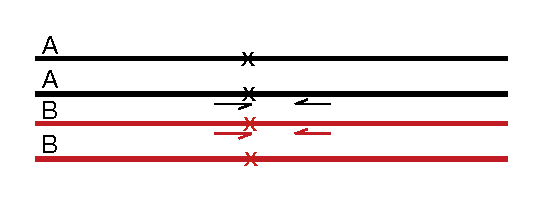
\includegraphics[width=1\textwidth]{PolyMarker/Figures/deletions/wt.pdf}
        \label{fig:poly:wt}
    \end{subfigure}
    ~
     \begin{subfigure}[b]{0.45\textwidth}
        \caption{}
        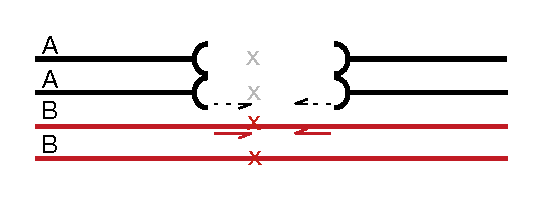
\includegraphics[width=1\textwidth]{PolyMarker/Figures/deletions/homM4.pdf}
        \label{fig:poly:homM4}
    \end{subfigure}
    \begin{subfigure}[b]{0.3\textwidth}
        \caption{}
        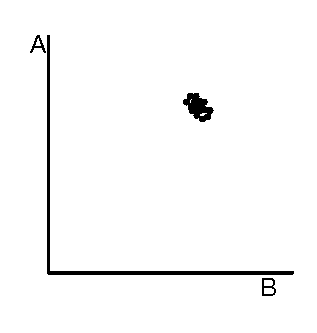
\includegraphics[width=1\textwidth]{PolyMarker/Figures/deletions/homFalse.pdf}
        \label{fig:poly:homFalse}
    \end{subfigure}
    ~
    \begin{subfigure}[b]{0.3\textwidth}
        \caption{}
        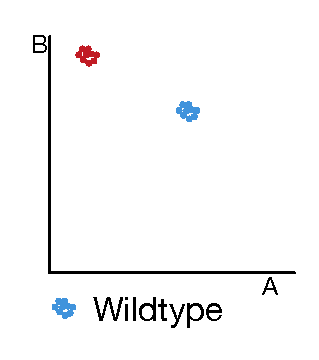
\includegraphics[width=1\textwidth]{PolyMarker/Figures/deletions/homReal.pdf}
        \label{fig:poly:homReal}
    \end{subfigure}
    \caption{KASP assays to validate homozygous deletions. (\subref{fig:poly:wt}) Primer positions for wildtype. (\subref{fig:poly:homM4}) Primer positions on  homozygous deletion on $M_{4}$ (\subref{fig:poly:homFalse} Heterozygous amplification on wildtype, including both homoeologues. (\subref{fig:poly:homReal}) Homozygous amplification on deletion line, only the non-deletad homoeologue is amplified. }
\end{figure}

On some of the TILLING mutant lines long deletions were detected \citep{Krasileva2016}.
To validate the deletions is possible to use KASP assays to produce primers that amplify homoeologues.  
PolyMarker was modified to search for variations across homoeologues to select a common primer that will amplify two genomes (Figure \ref{fig:poly:wt}, \subref{fig:poly:homM4}). 
On lines without the targeted deletion, the amplification correspond to an homozygous assay (Figure \ref{fig:poly:homFalse}).  
When a deletion is present the results of the assay look like an homozygous sample, with the intensity of the assay towards the the conserved homoeologue (Figure \ref{fig:poly:homReal}).
A set of KASP assays for the the deletions and mutations located on the same chromosome where designed to validate 11 homozygous deletions on $M_{4}$ plants. 
In all cases the segregation of the mutations was as expected, except for a predicted heterozygous mutation that was called as homozygous. 
Also, all the KASP assays that contained a deletion were called homozygous, as expected. 
To ensure that the calls didn't come from a single cluster, 4 wildtype plants were genotyped and the markers for deletions where called as heterozygous. 
An example of a validated deletion, with the calls for each individual is shown on Table \ref{app:poly:homDelCad0423}.

\subsection{PolyMarker public web service}
To make PolyMarker accessible to the community, a web server that allow the submission of SNPs was developed. 
The web interface consists on two virtual machines, one with a web facing interface that stores the queries, and a dedicated node to submit jobs to an HPC cluster.
The on-line interface further simplifies the design of KASP assays, a process that used to take a couple of weeks now is done in a couple of hours. 
Since the release of the public service in July 2014 until August 2016, 1,739 requests to PolyMarker have been done. 
%TODO: Does this sounds like too much marketing? 


\subsection{Genotyping of \textit{Puccinia 
striiformis} f. sp. \textit{tritici} isolates.}
In \cite{Hubbard2015}, \textit{Puccinia striiformis} f. sp. \textit{tritici} (PST) isolates were sequenced and assigned to clusters, according to their genotype.
The clusters are useful to monitor the changes in the pathogen population, which can be used to predict if certain wheat lines will be resistant to the isolates in the field. 
PolyMarker was used to design primers for PST, using the assembly PST-130 \citep{Cantu2011}.
Out of 15 assays 11 can be used to identify to which cluster of isolates a sample is likely to belong, Supplemental Table \ref{app:PolyMarkerPST}.


\section{Discussion}

PolyMarker is a tool that was born as part of the validation of the SNPs found in Chapter \ref{yr15}. 
Originally, the primer design was ought to be done manually, a slow, error-prone and, repetitive process. 
The steps require the use of several bioinformatics tools, but once I figured out the steps I decided to automate the process. 
Since designing genome-specific primers is a common task in wheat research and breeding, the community showed interest on the tool and I decided to refine it and make it open source. 
PolyMarker has been used successfully in several projects and it even allowed the novel use of KASP assays to validate long deletions in polyploids. 

% The mask generated by PolyMarker enabled the identification of putative homoeologous variants (between genomes as opposed to varietal SNPs) which were present in the data set, but that were not identified previously. By exploiting the latest genomic resources in wheat, PolyMarker increases the likelihood of generating codominant SNP assays that are required for commercial MAS programmes and genotyping of F2 mapping populations like the one used in this study. 


The ideas behind PolyMarker had been taken by other projects like the scripts described in \cite{Ma2015} and the corresponding web interface, GSP \citep{Wang2016}. 
Briefly, GSP does a blast search to find all the homoeologus regions and provides a diagram with the bases that are genome specific. 
It then allows the user to select a primer pair according to the constrains for the experiment, like product size. 
The advantage over PolyMarker is that it allows to pick arbitrary primers, at the cost of having a step for manual selection of the pair. 
Recently, LGC also developed a program (MAGICBOX) that require a SNP sequence, does the alignment and selects primers with a genome specific anchor. 
As PolyMarker, it produces a local alignment with the genome-specific bases \citep{Curry2016}. 

%The ideas behind PolyMarker had 
%Magic box from LGC https://www.lgcgroup.com/LGCGroup/media/PDFs/Our%20science/Genomics/PAG2016/improving-genome-specific-kasp-markers-for-hexaploid-wheat-magicbox-automated-design-pipeline.pdf


The current web interface of PolyMarker is limited to KASP assays, however the command line version is more flexible and has been used to design primers for PCR amplicons, capillary sequencing and on other organisms. 


As new references of wheat come available, PolyMarker should be updated to work with pseudomolecules and the web interface updated accordingly.  

%Remarks on the importance of getting the primers right, and the time saved by automating the primer selection. Also mention other primer design tools that have been inspired by polymarker: \cite{Ma2015}, \cite{Wang2016}

 


